\PassOptionsToPackage{quiet}{fontspec}
\documentclass[UTF8]{ctexart}
\usepackage{titlesec}
\usepackage{fancyhdr}
\usepackage{geometry}
\usepackage{listings}
\usepackage{xcolor}
\usepackage{graphicx}
\usepackage{amsmath}  % 提供了高级数学公式环境
\usepackage{amsfonts} % 提供数学字体
\usepackage{amssymb}  % 提供额外的数学符号

\geometry{left=1.0in,right=1.0in,top=0.3in,bottom=0.3in}

\pagestyle{fancy}
\fancyhf{} % 清空当前的页眉和页脚
\fancyfoot[C]{\thepage} % 页脚中间显示页码

\ctexset{
    section={%
        format=\raggedright\Large\bfseries,
        afterskip=10pt,
    },
    subsection={%
        format=\raggedright\normalsize,
        afterskip=8pt,
    }
}

\lstset{
    language=C++, 
    basicstyle=\ttfamily\small, % 字体样式和大小
    keywordstyle=\color{blue}, % 关键字颜色
    commentstyle=\color{gray}, % 注释颜色
    stringstyle=\color{red}, % 字符串颜色
    numbers=left, % 显示行号
    numberstyle=\tiny\color{gray}, % 行号样式
    frame=single, % 代码框
    breaklines=true, % 自动换行
    captionpos=b % 标题位置
}


\begin{document}
\title{\vspace{0cm}最大互斥集合问题实验报告}
\author{程远2234412848}
\date{}
\maketitle

\section{问题描述}
给定一个 $1000 \times 20$ 的矩阵 $\text{matrix}$,其中每个元素均为 $0$ 或 $1$。设计一个算法,从中找出两组互斥的列集合 $A$ 和 $B$,使得两组集合包含的列数总和最大。两组集合互斥的定义是:任意一行中,$A$ 中的任意列与 $B$ 中的任意列不能同时为 $1$。

\subsection*{输入格式}
一个包含 $1000 \times 20$ 的矩阵 $\text{matrix}$。

\subsection*{输出格式}
两行输出:
\begin{itemize}
    \item 第一行输出集合 $A$ 的所有元素(列索引,从 $0$ 开始),以空格分隔。
    \item 第二行输出集合 $B$ 的所有元素,格式同上。
\end{itemize}
若找不到符合条件的非空集合,则输出两行空行。

\section{问题分析}
本问题是一个组合优化问题,涉及子集选择与互斥关系判定。难点包括:
\begin{enumerate}
    \item \textbf{互斥性判定}:需要快速判断两列是否互斥。
    \item \textbf{优化目标}:找到包含列数最多且互斥的集合。
    \item \textbf{计算量控制}:在 $2^{20}$ 种子集组合中选择最佳方案。
\end{enumerate}

通过预处理互斥关系和列总和,可以显著加速搜索过程。同时,利用位运算枚举所有可能的集合组合。

\section{算法设计}
算法分为以下几步:
\begin{enumerate}
    \item \textbf{互斥关系预处理}:遍历矩阵每一行,判定任意两列是否互斥,并存储在二维布尔数组 $\text{judge}[][]$ 中。
    \item \textbf{列总和预处理}:计算每列中 $1$ 的总数,存储在数组 $\text{sum}[]$ 中,用于快速计算子集总和。
    \item \textbf{枚举子集}:利用位运算枚举所有可能的列集合 $A$。
    \item \textbf{构造集合 $B$}:根据 $\text{judge}[][]$ 判断剩余列是否与 $A$ 互斥,并构造集合 $B$。
    \item \textbf{更新最优解}:比较当前组合是否优于历史最佳组合,若是则更新最佳解。
\end{enumerate}

\section{算法实现}
以下是算法的完整实现代码:
\begin{lstlisting}
    #include <iostream>
    #include <vector>
    using namespace std;
    
    const int M = 25, N = 1010; // M 为列数上限,N 为行数上限
    bool judge[M][M];           // judge[i][j] 记录列 i 和列 j 是否互斥
    int a[N][M];                // a[i][j] 记录输入矩阵的元素
    int sum[M];                 // sum[i] 存储第 i 列中 1 的总和
    vector<int> best_set_a, best_set_b; // 存储当前最优的集合 A 和 B
    int asum, bsum, eps = 100, tc; // asum 和 bsum 为当前 A 和 B 的元素个数,eps 用于平衡解的差异,tc 为最大列总数
    
    // 判断列 x 和列 y 是否互斥
    bool isCompatible(int x, int y) 
    {
        for (int i = 0; i < 1000; i++) 
        {
            if (a[i][x] + a[i][y] == 2) 
            {
                return false;
            }
        }
        return true;
    }
    
    // 初始化 judge 数组,记录所有列之间的互斥关系
    void initJudge() 
    {
        for (int i = 0; i < 20; i++) 
        {
            for (int j = i + 1; j < 20; j++) 
            {
                if (isCompatible(i, j)) 
                {
                    judge[i][j] = judge[j][i] = true;
                }
            }
        }
    }
    
    // 计算每列中 1 的总和并存储在 sum 数组中
    void sumOfCol() 
    {
        for (int i = 0; i < 20; i++) 
        {
            int res = 0;
            for (int j = 0; j < 1000; j++) 
            {
                res += a[j][i];
            }
            sum[i] = res;
        }
    }
    
    // 判断当前组合是否优于历史最佳组合
    bool isBetter(const vector<int>& a, const vector<int>& b) 
    {
        if (a.size() > b.size()) 
        {
            return true;
        }
        if (a.size() < b.size()) 
        {
            return false;
        }
        for (size_t i = 0; i < min(a.size(), b.size()); i++) 
        {
            if (a[i] < b[i]) 
            {
                return true;
            }
            if (a[i] > b[i]) 
            {
                return false;
            }
        }
        return false;
    }
    
    // 更新当前的最优解
    void update(const vector<int>& set_a, const vector<int>& set_b) 
    {
        best_set_a = set_a;
        best_set_b = set_b;
        tc = set_a.size() + set_b.size(); // 更新最大列总数
    }
    
    // 主函数
    int main() 
    {
        // 输入矩阵数据
        for (int i = 0; i < 1000; i++) 
        {
            for (int j = 0; j < 20; j++) 
            {
                cin >> a[i][j];
            }
        }
    
        // 预处理 judge 和 sum 数组
        initJudge();
        sumOfCol();
    
        // 枚举所有可能的子集 A
        for (int i = 1; i < (1 << 20); i++) 
        {
            vector<int> set_a, set_b;
    
            // 构造子集 A
            for (int k = 0; k < 20; k++) 
            {
                if (i & (1 << k)) 
                {
                    set_a.push_back(k);
                }
            }
    
            // 根据互斥关系构造集合 B
            for (int k = 0; k < 20; k++) 
            {
                if (set_a.empty()) 
                {
                    continue;
                }
                bool compatible = true;
                for (int col : set_a) 
                {
                    if (!judge[col][k]) 
                    {
                        compatible = false;
                        break;
                    }
                }
                if (compatible) 
                {
                    set_b.push_back(k);
                }
            }
    
            // 判断当前组合是否优于历史最佳
            if (set_a.size() + set_b.size() > tc || 
                (set_a.size() + set_b.size() == tc && isBetter(set_a, best_set_a))) 
            {
                update(set_a, set_b);
            }
        }
    
        // 输出最优解
        if (!best_set_a.empty()) 
        {
            for (int col : best_set_a) 
            {
                cout << col << " ";
            }
            cout << endl;
            for (int col : best_set_b) 
            {
                cout << col << " ";
            }
            cout << endl;
        } 
        else 
        {
            cout << endl << endl; // 如果没有找到非空解,输出两行空行
        }
    
        return 0;
    }    
\end{lstlisting}

\section{复杂度分析}
假设矩阵大小为 $m \times n$,我们分析算法的时间和空间复杂度。

\subsection*{1. 预处理复杂度}
\begin{enumerate}
    \item \textbf{互斥关系判断}:
    \begin{itemize}
        \item 遍历所有列对 $(i, j)$,判断它们是否互斥。
        \item 每对列需要遍历 $m$ 行。
        \item 列对总数为 $\binom{n}{2} = \frac{n(n-1)}{2}$。
    \end{itemize}
    时间复杂度:$O(m \cdot n^2)$。

    \item \textbf{列总和计算}:
    \begin{itemize}
        \item 遍历所有 $m \times n$ 的元素,计算每列中 $1$ 的总数。
    \end{itemize}
    时间复杂度:$O(m \cdot n)$。
\end{enumerate}

\subsection*{2. 枚举子集复杂度}
\begin{enumerate}
    \item \textbf{子集枚举}:
    \begin{itemize}
        \item 所有列的子集总数为 $2^n$。
        \item 每个子集的构造需要 $O(n)$。
    \end{itemize}
    时间复杂度:$O(2^n \cdot n)$。

    \item \textbf{构造集合 $B$}:
    \begin{itemize}
        \item 对于每个子集 $A$,需要检查剩余列是否与 $A$ 的所有列互斥。
        \item 最坏情况下,每列需要与 $A$ 中的 $n$ 列比较。
    \end{itemize}
    时间复杂度:$O(2^n \cdot n^2)$。
\end{enumerate}

\subsection*{3. 总复杂度}
综合上述分析,总时间复杂度为:
\[
O(m \cdot n^2 + 2^n \cdot n^2)
\]
其中:
\begin{itemize}
    \item $O(m \cdot n^2)$ 是预处理复杂度。
    \item $O(2^n \cdot n^2)$ 是子集枚举和构造集合的复杂度。
\end{itemize}

\subsection*{4. 空间复杂度}
\begin{itemize}
    \item 存储输入矩阵需要 $O(m \cdot n)$ 的空间。
    \item 存储互斥关系矩阵需要 $O(n^2)$ 的空间。
    \item 存储子集和中间结果需要 $O(n)$ 的空间。
\end{itemize}
总空间复杂度为:
\[
O(m \cdot n + n^2)
\]

\section{运行结果}
通过moodle上所有用例
\begin{figure}[htbp]
    \centering
    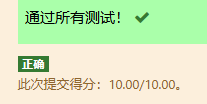
\includegraphics[width=0.8\textwidth]{moodle.png}
\end{figure}

\section*{剪枝优化和位运算优化}

\subsection{剪枝优化}
当前算法会枚举所有 $2^n$ 种可能的子集,其中许多子集在构造时已经可以判断无法超过历史最优解,继续搜索会浪费计算资源。
在子集枚举和集合构造时,提前判断某些组合是否不可能成为最优解,直接跳过无效计算。

\paragraph{实现步骤}
\begin{enumerate}
    \item \textbf{子集枚举剪枝}:
    在枚举子集 $A$ 时,若 $|A| + (\text{未选列数}) \leq \text{当前最优列数总和}$,直接跳过。
    \item \textbf{冲突检测剪枝}:
    在构造集合 $B$ 时,若某列与 $A$ 中任意列冲突,则立即跳过。
\end{enumerate}

\paragraph{剪枝的效果}
\begin{itemize}
    \item \textbf{时间复杂度}:剪枝后实际子集枚举复杂度从 $O(2^n)$ 降至近似 $O(k \cdot 2^n)$,其中 $k$ 为有效子集比例,远小于 1。
    \item \textbf{性能提升}:当 $n = 20$ 时,可能减少超过 50\% 的无效计算。
\end{itemize}

\subsection{位运算优化}
当前算法使用显式数组存储和操作集合,对于小规模问题可以用位运算代替以进一步提高效率。
\paragraph{优化方法}
\begin{enumerate}
    \item 使用整数的二进制位表示子集。例如,整数 $5$ (\texttt{101}) 表示子集包含第 $0$ 和第 $2$ 列。
    \item 用按位与操作快速判断列是否互斥。例如,$(\text{mask} \, \& \, \text{judge}[k]) == 0$ 可判断子集与列 $k$ 是否互斥。
\end{enumerate}

\paragraph{实现步骤}
\begin{itemize}
    \item 用整数代替显式数组表示集合 $A$ 和 $B$。
    \item 用位运算代替集合遍历和更新操作。
\end{itemize}

\paragraph{位运算的效果}
\begin{itemize}
    \item \textbf{时间复杂度}:集合操作从 $O(n)$ 降至 $O(1)$。
    \item \textbf{性能提升}:在 $n = 20$ 时,子集操作的时间开销显著降低。
\end{itemize}

\end{document}